\begin{figure}
    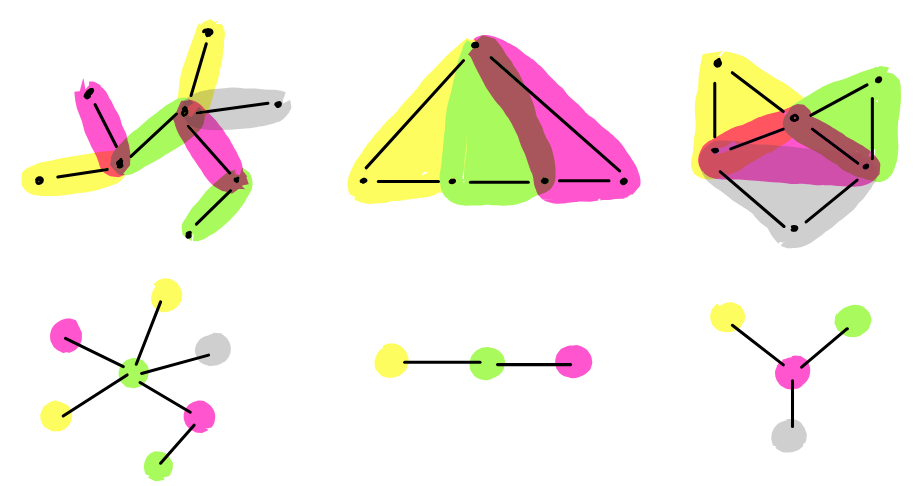
\includegraphics[width=\textwidth]{figures/treewidth-example.png}
    \caption{Examples of treewidth. (a) A tree has treewidth 1. (b) A cycle has treewidth 2. (c) A random graph with treewidth 2. For each example, the graph with its bags is shown at the top, and the tree decomposition of the bags is depicted at the bottom. \todo{add different colors for each bag}}
    \label{fig:treewidth-example}
\end{figure}